%!xelatex = 'xelatex --halt-on-error %O %S'

\documentclass{seuer}
% \usepackage[UTF8]{ctex}

\begin{document}

% 标题,作者
\emptitle{RANSAC实验报告}
\empauthor{朱启鹏}

% 奇数页页眉 % 请在这里写出第一作者以及论文题目
\fancyhead[CO]{{\footnotesize 朱启鹏: RANSAC实验报告}}


%%%%%%%%%%%%%%%%%%%%%%%%%%%%%%%%%%%%%%%%%%%%%%%%%%%%%%%%%%%%%%%%
% 关键词 摘要 首页脚注
%%%%%%%%关键词
% \Keyword{关键词, 很关键的词, 十分关键的词, 有一些关键的词, 大关键词}
\twocolumn[
\begin{@twocolumnfalse}
\maketitle

%%%%%%%%摘要
% \begin{empAbstract}
% 摘要内容,小五号宋体,不超过500字。简要概述主要实验内容和结果。要求:论文的基本信息和要点都应该出现在摘要里;使用标准精确的词汇和语言,清晰紧凑地概述客观事实;摘要的整体结构严谨、思路清楚,基本素材组织合理。英文摘要与中文内容一致。英文摘要须与中文内容一致,被动语态、现在时。字号为小五New Times Roman。论文的中、英文摘要是国内外数据库收录的主要内容,所以摘要的内容直接影响到该论文能否被收录及收录后被引用的情况,作者应给予高度重视。关键词为经过规范化处理的词语或短语,数量一般为3~5个。同一篇文章的中英文关键词的内容和顺序应一致。
% \end{empAbstract}

%%%%%%%%首页角注,依次为实验时间、报告时间、学号、email
\empfirstfoot{2021-10-24}{2021-10-29}{58119304}{213191670@seu.edu.cn}
\end{@twocolumnfalse}
]
%%%%%%%%!首页角注可能与正文重叠,请通过调整正文中第一页的\enlargethispage{-3.3cm}位置手动校准正文底部位置:
%%%%%%%%%%%%%%%%%%%%%%%%%%%%%%%%%%%%%%%%%%%%%%%%%%%%%%%%%%%%%%%%
%  正文由此开始
\wuhao 
%  分栏开始
\section{算法介绍}
\subsection{训练}
(1)定义样本点集 $\mathcal{M}$,对其进行均匀采样,可以得到样本点子集 $\mathcal{N}$:
\begin{equation}\label{EQ1}
\mathcal{N} = \{(x_1, y_1), (x_2, y_2), ..., (x_i, y_i) ...\}
\end{equation}
\begin{equation}\label{EQ1}
   i=1 , 2...p,\ (p=|\mathcal{N}|)
\end{equation}
(2)在 $\mathcal{N}$ 上进行拟合线性模型:

具体拟合过程如下:

定义直线:
\begin{equation}\label{EQ1}
  \begin{aligned}
  ax+by=d,\\ 
  \text{s.t.} \quad a^2+b^2=1
  \end{aligned}
\end{equation}

定义点到直线的距离:
\begin{equation}\label{EQ1}
  \begin{array}{ll}
  \text{distance}=\frac{|ax_i+by_i-d|}{\sqrt{a^2+b^2}}=|ax_i+by_i-d|,\\ 
  \text{s.t.} \quad (x_i, y_i)\in \mathcal{N}
  \end{array}
\end{equation}

定义目标函数:
\begin{equation}\label{EQ1}
  \begin{aligned}
  E=\sum_{i=1}^{n}(ax_i+by_i-d)^2\\ 
  \end{aligned}
\end{equation}

令目标函数参数$d$的一阶偏导数为0:
\begin{equation}\label{EQ1}
  \begin{aligned}
  \frac{\partial E}{\partial d}=\sum_{i=1}^{n}-2\left(a x_{i}+b y_{i}-d\right)=0
  \end{aligned}
\end{equation}

得到$d$的表达式:
\newpage
\begin{equation}\label{EQ1}
  \begin{aligned}
    d=\frac{a}{n} \sum_{i=1}^{n} x_{i}+\frac{b}{n} \sum_{i=1}^{n} y_{i}=a \bar{x}+b \bar{y}\\
  \end{aligned}
\end{equation}

将(6))代入(5)式:
\begin{equation}\label{EQ1}
  \begin{array}{ll}
    E=\sum_{i=1}^{n}\left(a\left(x_{i}-\bar{x}\right)+b\left(y_{i}-\bar{y}\right)\right)^{2}\\
    \quad=\left\|\left[\begin{array}{cc}
    x_{1}-\bar{x} & y_{1}-\bar{y} \\
\vdots & \vdots \\
x_{n}-\bar{x} & y_{n}-\bar{y}
\end{array}\right]\left[\begin{array}{c}
a \\
b
\end{array}\right]\right\|^{2}\\
\quad=(U N)^{T}(U N) 
  \end{array}
\end{equation}

令$E$ 对 $N$ 的一阶偏导值为0:
\begin{equation}\label{EQ1}
  \begin{array}{ll}
    \frac{d E}{d N}=2\left(U^{T} U\right) N=0
  \end{array}
\end{equation}

$A$ 是一个 $n \times n$ 的矩阵, $x$ 是一个非零向量, 

如果:
\begin{equation}\label{EQ1}
  \begin{array}{ll}
    A x=\lambda x, \quad x \neq 0
  \end{array}
\end{equation}

那么我们$x$的解就是$A$的特征向量。

利用式(10),我们可以对式(9)进行求解$N$:

\begin{equation}\label{EQ1}
  \begin{array}{ll}
    (U^TU)N=0,\\
    \|N\|^2=1
  \end{array}
\end{equation}

对于给定$U$如下:
\begin{equation}\label{EQ1}
  \begin{array}{ll}
    U=\left[\begin{array}{cc}
      x_{1}-\bar{x} & y_{1}-\bar{y} \\
      \vdots & \vdots \\
      x_{n}-\bar{x} & y_{n}-\bar{y}
      \end{array}\right]
  \end{array}
\end{equation}

最终求解的$N$是$U^TU$的单位特征向量
\begin{equation}\label{EQ1}
  \begin{array}{ll}
    N=\left[\begin{array}{cc}
      a\\
      b
      \end{array}\right]
  \end{array}
\end{equation}

(3)利用拟合好的模型,统计除样本点外的点集$\mathcal{Q}$中有多少内点:
\begin{equation}\label{EQ1}
  \mathcal{Q}=\mathcal{N}-\mathcal{M}
\end{equation}

对于内点,我们可以给出以下定义:
\begin{equation}\label{EQ1}
  \begin{array}{ll}
    (x_i,y_i)\in\mathcal{P}_{\text{inlier}},\quad \text{if distance}(x_i,y_i)<\theta 
  \end{array}
\end{equation}

其中$\mathcal{P}_{\text{inlier}}$是一个内点集合,$\theta$是预先设置好的阈值

如果统计出的内点数大于$\epsilon$,$\epsilon$是预先设置好的一个阈值,那么这个模型可以被保留。接着我们在$\mathcal{P}_{\text{inlier}}$上,再对模型进行拟合

(4)重复(1)-(3)$K$ 次,其中 $K$ 是预先设置好的参数

(5)对队列中所有保留的模型都进行评估,输出评估效果最好的模型:
\begin{equation}\label{EQ1}
  \text{score}=\frac{\text{numbers of inlier  }}{numbers of points}
\end{equation}

\subsection{自适应调节最大迭代数$K$}
step1: 初始化参数, $K$为最大迭代数,$q$当前采样次数,$\phi$为当前最高内点率
\begin{equation}\label{EQ1}
  K=\infty, q = 0, r=\phi
\end{equation}

step2: 采样一个样本,通过拟合模型,计算出该模型的内点集$\mathcal{P}_{\text{inlier}}$,计算出内点率 $\hat{\phi} $,

step3: 如果:
\begin{equation}\label{EQ1}
  \begin{array}{ll}
    \hat{\phi}>\phi
  \end{array}
\end{equation}

那么进行更新:
\begin{equation}\label{EQ1}
  \begin{array}{ll}
  K :=\log (1-p) / \log \left(1-(1-e)^{s}\right)\\
  \phi := \hat{\phi}\\
  q := q + 1
  \end{array}
\end{equation}

step4: 如果 $K\leqslant  q$,重复step2-step3,否则结束循环输出 $K$

\section{实验}
\enlargethispage{-3.3cm}
在Windows10.0,12核CPU,7.85GB内存平台上,自主生成边缘点和噪声点。并在所生成的数据点上测试RANSAC算法的效果,以及不同参数对RANSAC的算法效率的影响

\subsection{硬件设备简述}
\begin{figure}[H]
  \centering
  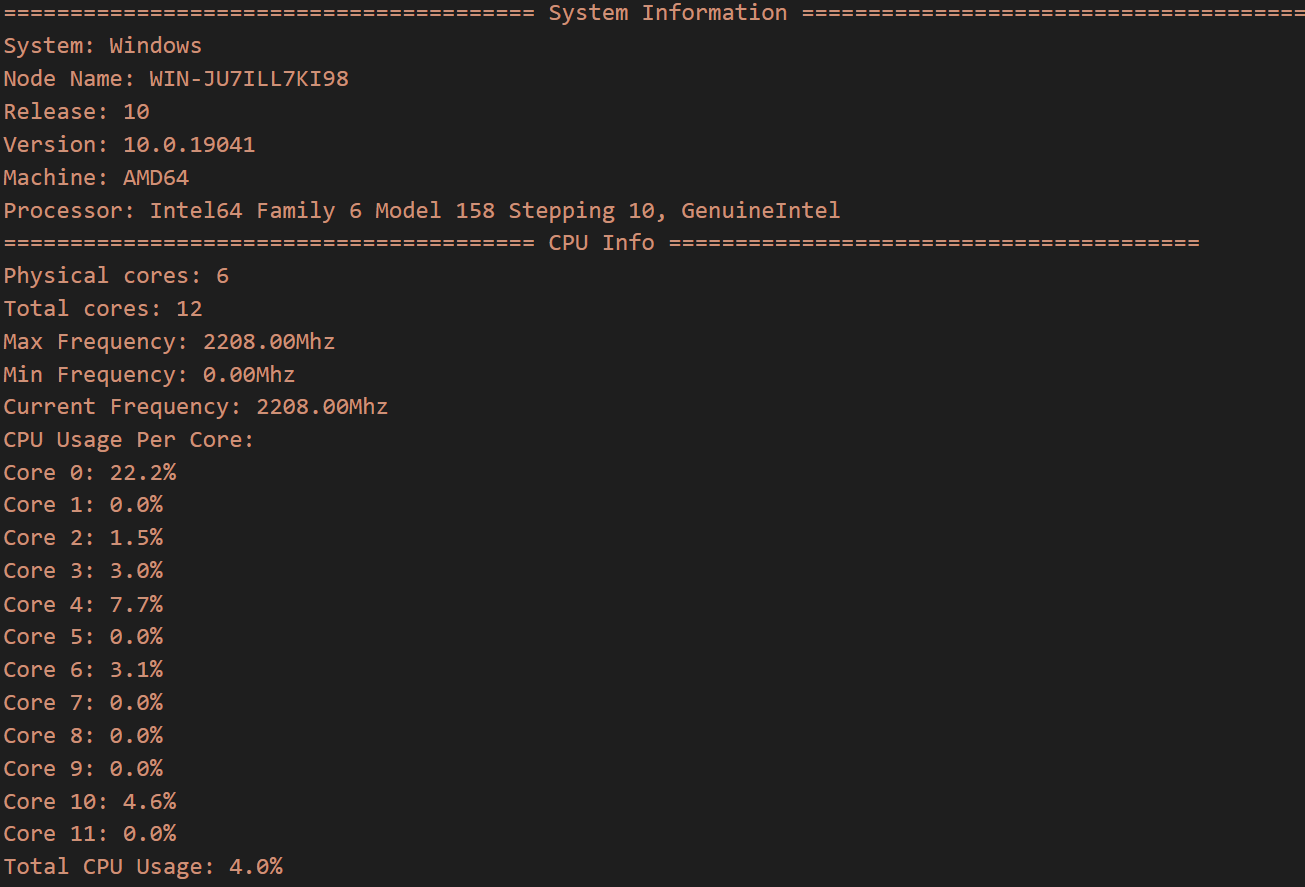
\includegraphics[width=0.8\linewidth]{./image/Info1.png}
  \caption{System Information and CPU Information} \label{fig:eg}
\end{figure}
\begin{figure}[H]
  \centering
  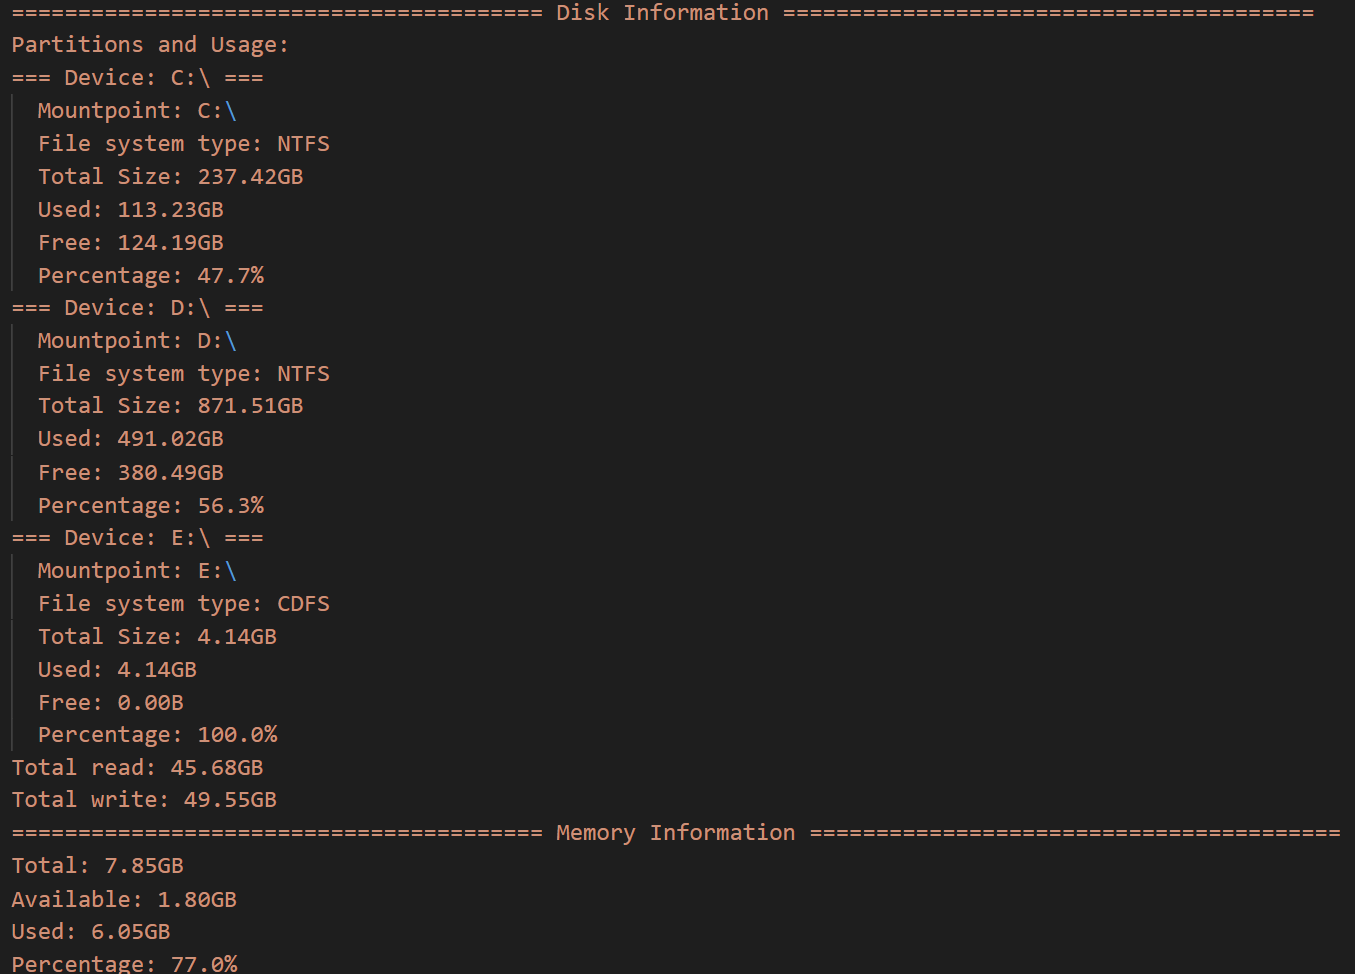
\includegraphics[width=0.8\linewidth]{./image/Info2.png}
  \caption{Disk Information and Memory Information} \label{fig:eg}
\end{figure}



\subsection{实验结果与分析}
\subsubsection{生成数据展示}
\begin{table}[h]
  \centering
  \captionnamefont{\wuhao\bf\heiti}
  \captiontitlefont{\wuhao\bf\heiti}
  \caption{参数列表} \label{tab:eg1}
  \liuhao
  \begin{tabular}{cccccc}
  \toprule
  {编号} &  {点数} & {噪音比例} & {斜率(k)} & {截距(b)} & {噪音类型}\\
  \midrule 
  1 & 10000 & 0.1 & -3.60 & 2.10 & Gaussian  \\
  2 & 10000 & 0.2 & -3.60 & 2.10 & Gaussian  \\
  3 & 10000 & 0.3 & -3.60 & 2.10 & Gaussian  \\
  \bottomrule
  \end{tabular}
\end{table}

中红色点是噪点,绿色点是正常点,黄绿色为原直线
从左到右分别是高斯噪音率0.1,0.2,0.3的数据图
\begin{figure}[H]
  \centering
  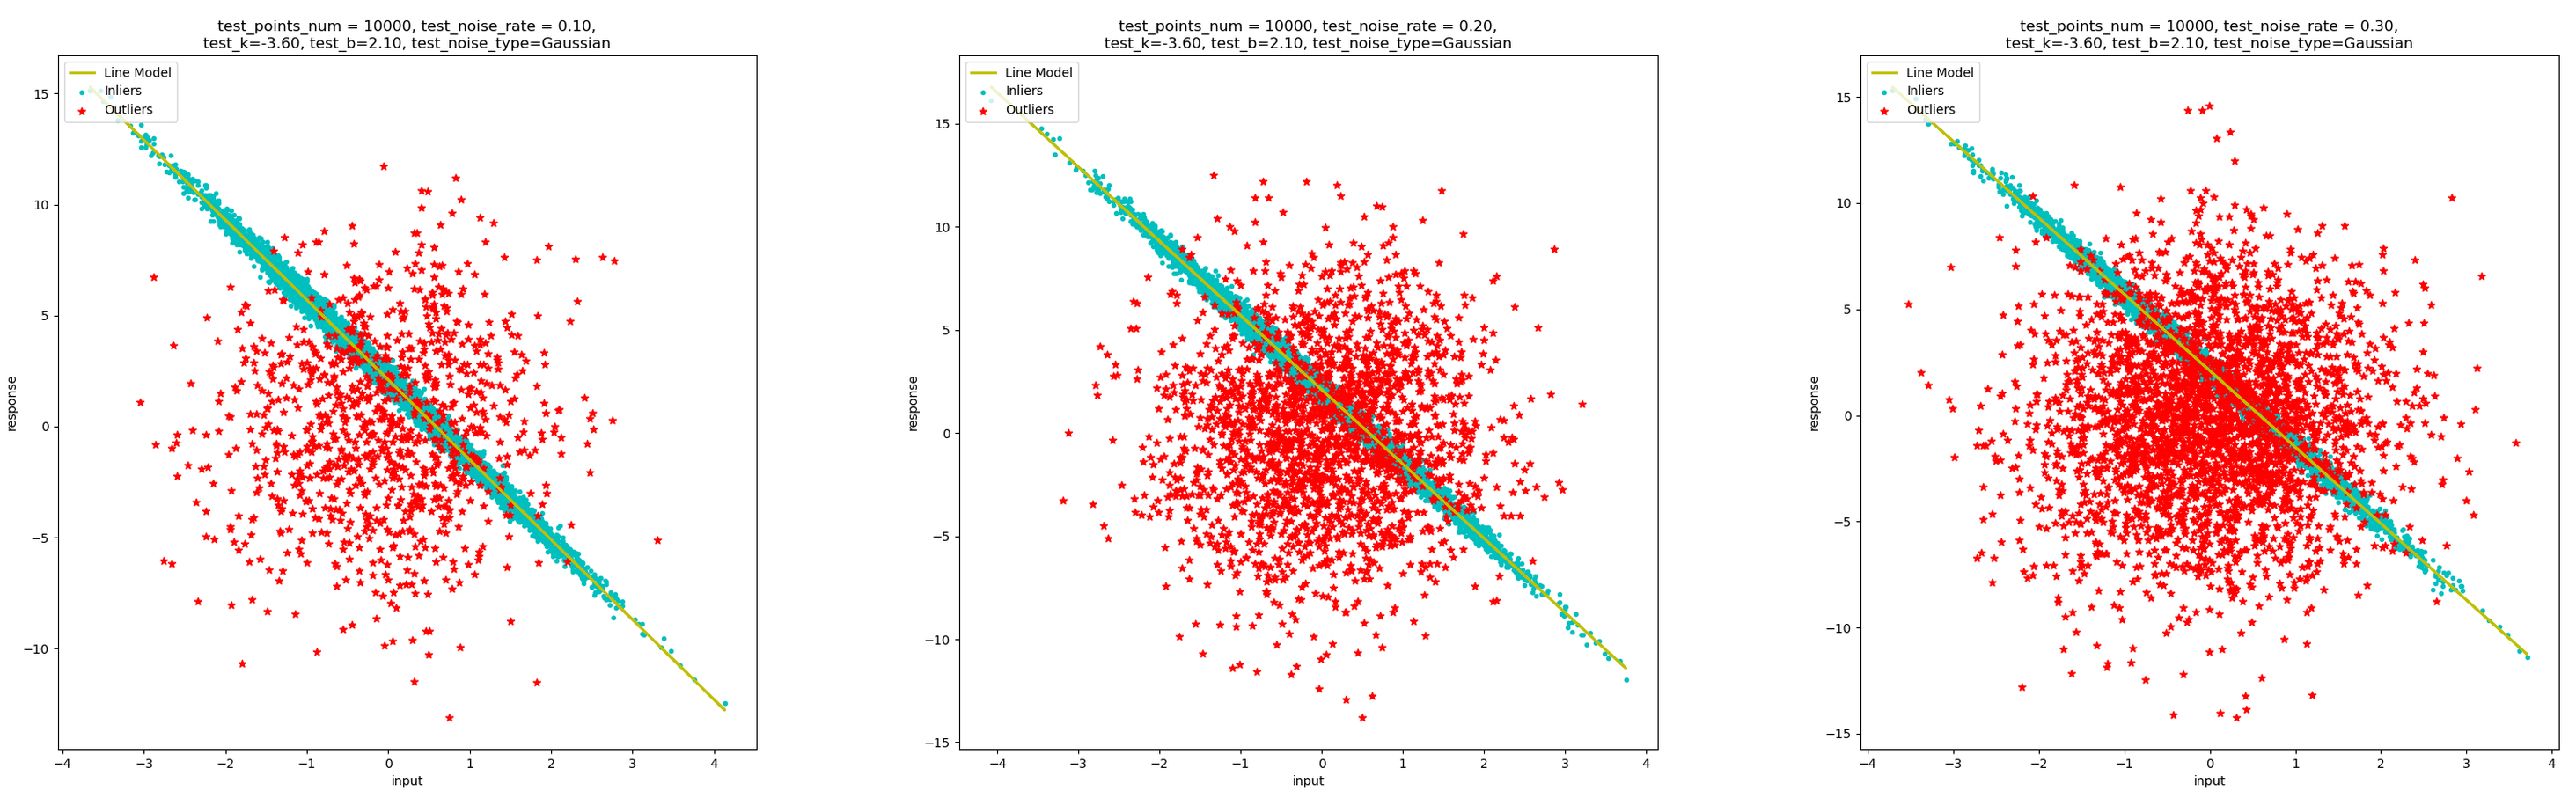
\includegraphics[scale=0.11]{./image/gen_data_Gaussian.png}
  \caption{10000 points with Gaussian Noise} \label{fig:eg}
\end{figure}
\begin{table}[h]
  \centering
  \captionnamefont{\wuhao\bf\heiti}
  \captiontitlefont{\wuhao\bf\heiti}
  \caption{参数列表} \label{tab:eg1}
  \liuhao
  \begin{tabular}{cccccc}
  \toprule
  {编号} &  {点数} & {噪音比例} & {斜率(k)} & {截距(b)} & {噪音类型}\\
  \midrule 
  1 & 10000 & 0.1 & -3.60 & 2.10 & Uniform  \\
  2 & 10000 & 0.2 & -3.60 & 2.10 & Uniform  \\
  3 & 10000 & 0.3 & -3.60 & 2.10 & Uniform  \\
  \bottomrule
  \end{tabular}
\end{table}

从左到右分别是均匀噪音率0.1,0.2,0.3的数据图
\begin{figure}[H]
  \centering
  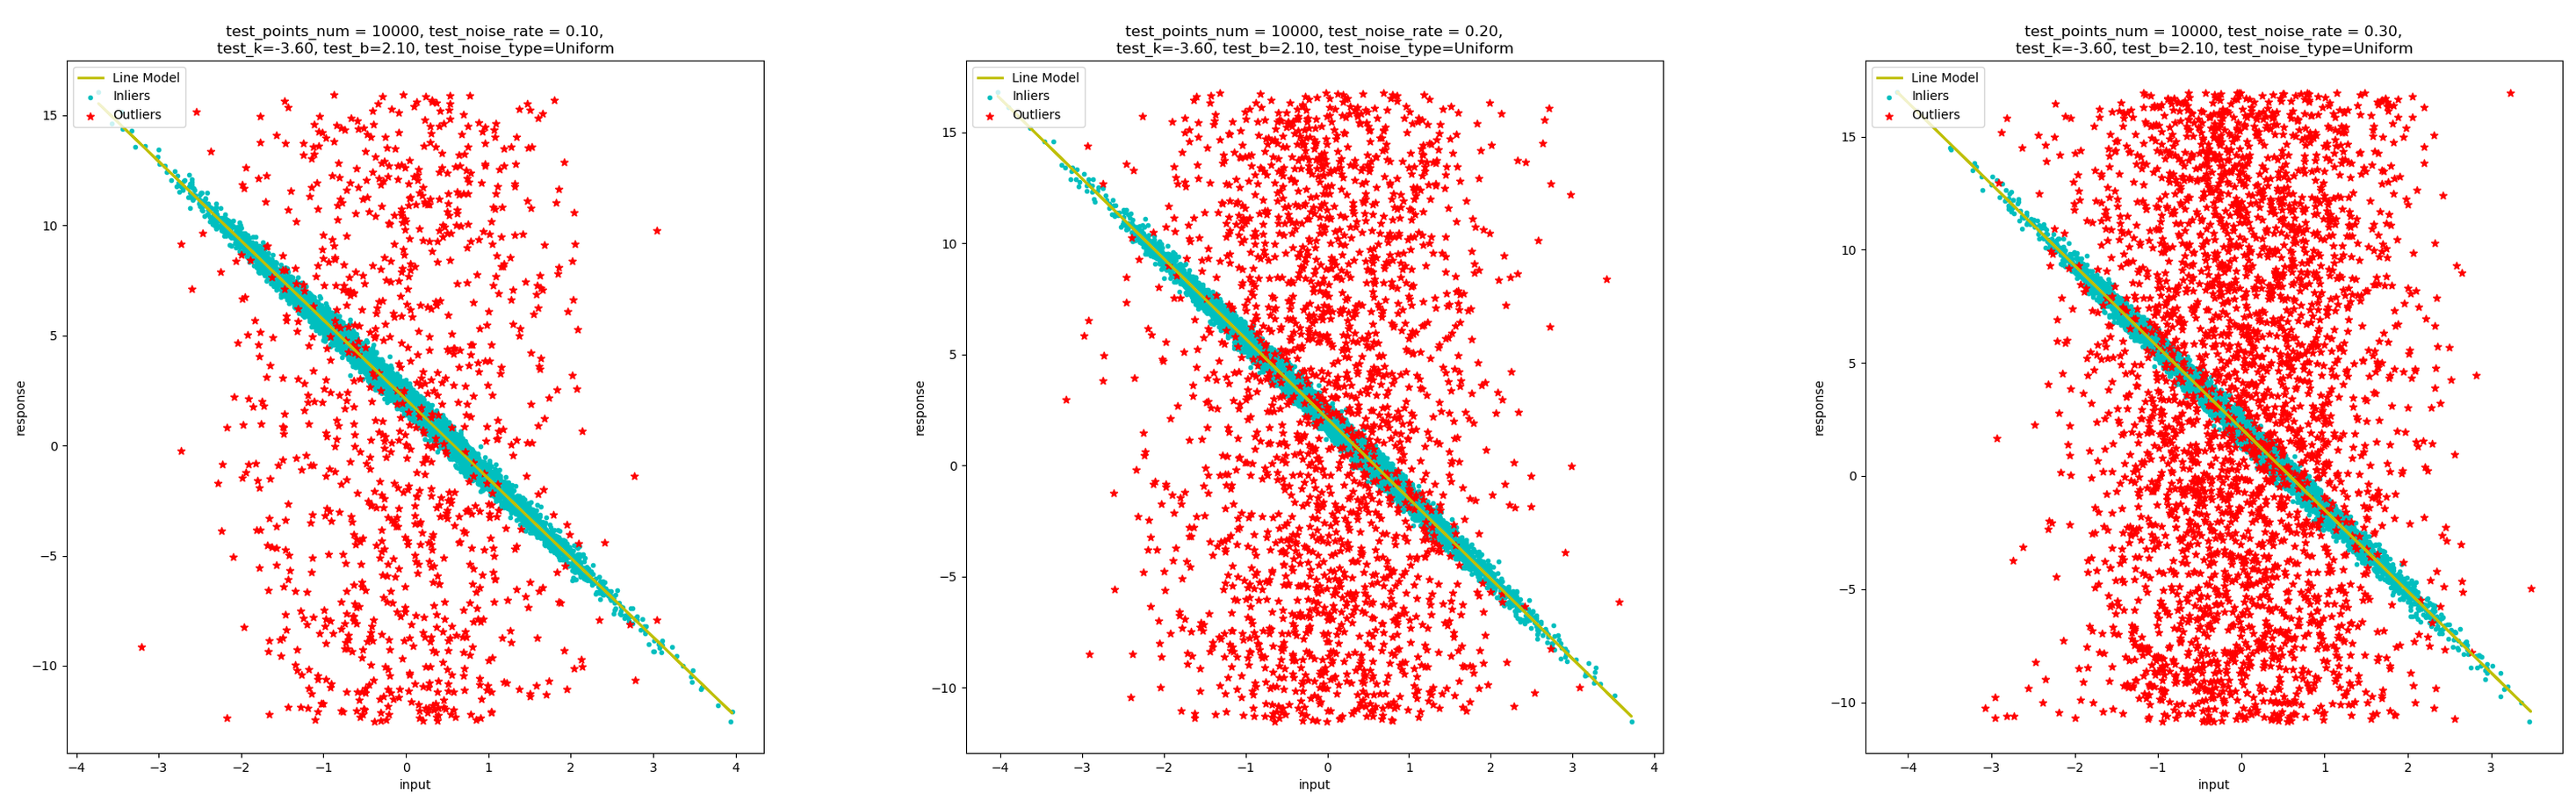
\includegraphics[scale=0.11]{./image/gen_data_Uniform.png}
  \caption{10000 points with Uniform Noise} \label{fig:eg}
\end{figure}
\subsubsection{RANSAC基于不同噪音率、噪音类型、阈值测试}
\begin{table}[h]
  \centering
  \captionnamefont{\wuhao\bf\heiti}
  \captiontitlefont{\wuhao\bf\heiti}
  \caption{默认参数列表} \label{tab:eg1}
  \liuhao
  \begin{tabular}{ccccc}
  \toprule
  {点数} & {噪音比例} & {斜率(k)} & {截距(b)} & {噪音类型}\\
  \midrule 
  3000 & 0.1 & 2.3 & 4.2 & Gaussian / Uniform\\
  \bottomrule
  \end{tabular}
\end{table}
\begin{table}[h]
  \centering
  \captionnamefont{\wuhao\bf\heiti}
  \captiontitlefont{\wuhao\bf\heiti}
  \caption{续表3} \label{tab:eg1}
  \liuhao
  \begin{tabular}{cccccccccc}
  \toprule
  {采样个数} & {最大迭代数} & {内点阈值} & {模型判定阈值}\\
  \midrule 
  30 & 90 & 0.50 & 2550 \\
  \bottomrule
  \end{tabular}
\end{table}

\paragraph{不同噪音率,RANSAC拟合效果比较}
图中红色点是噪点,绿色点是正常点,黄绿色为原直线,黄色为拟合直线

从左到右分别是在高斯噪音率0.1,0.2,0.3的数据集上拟合的效果图
\begin{figure}[H]
  \centering
  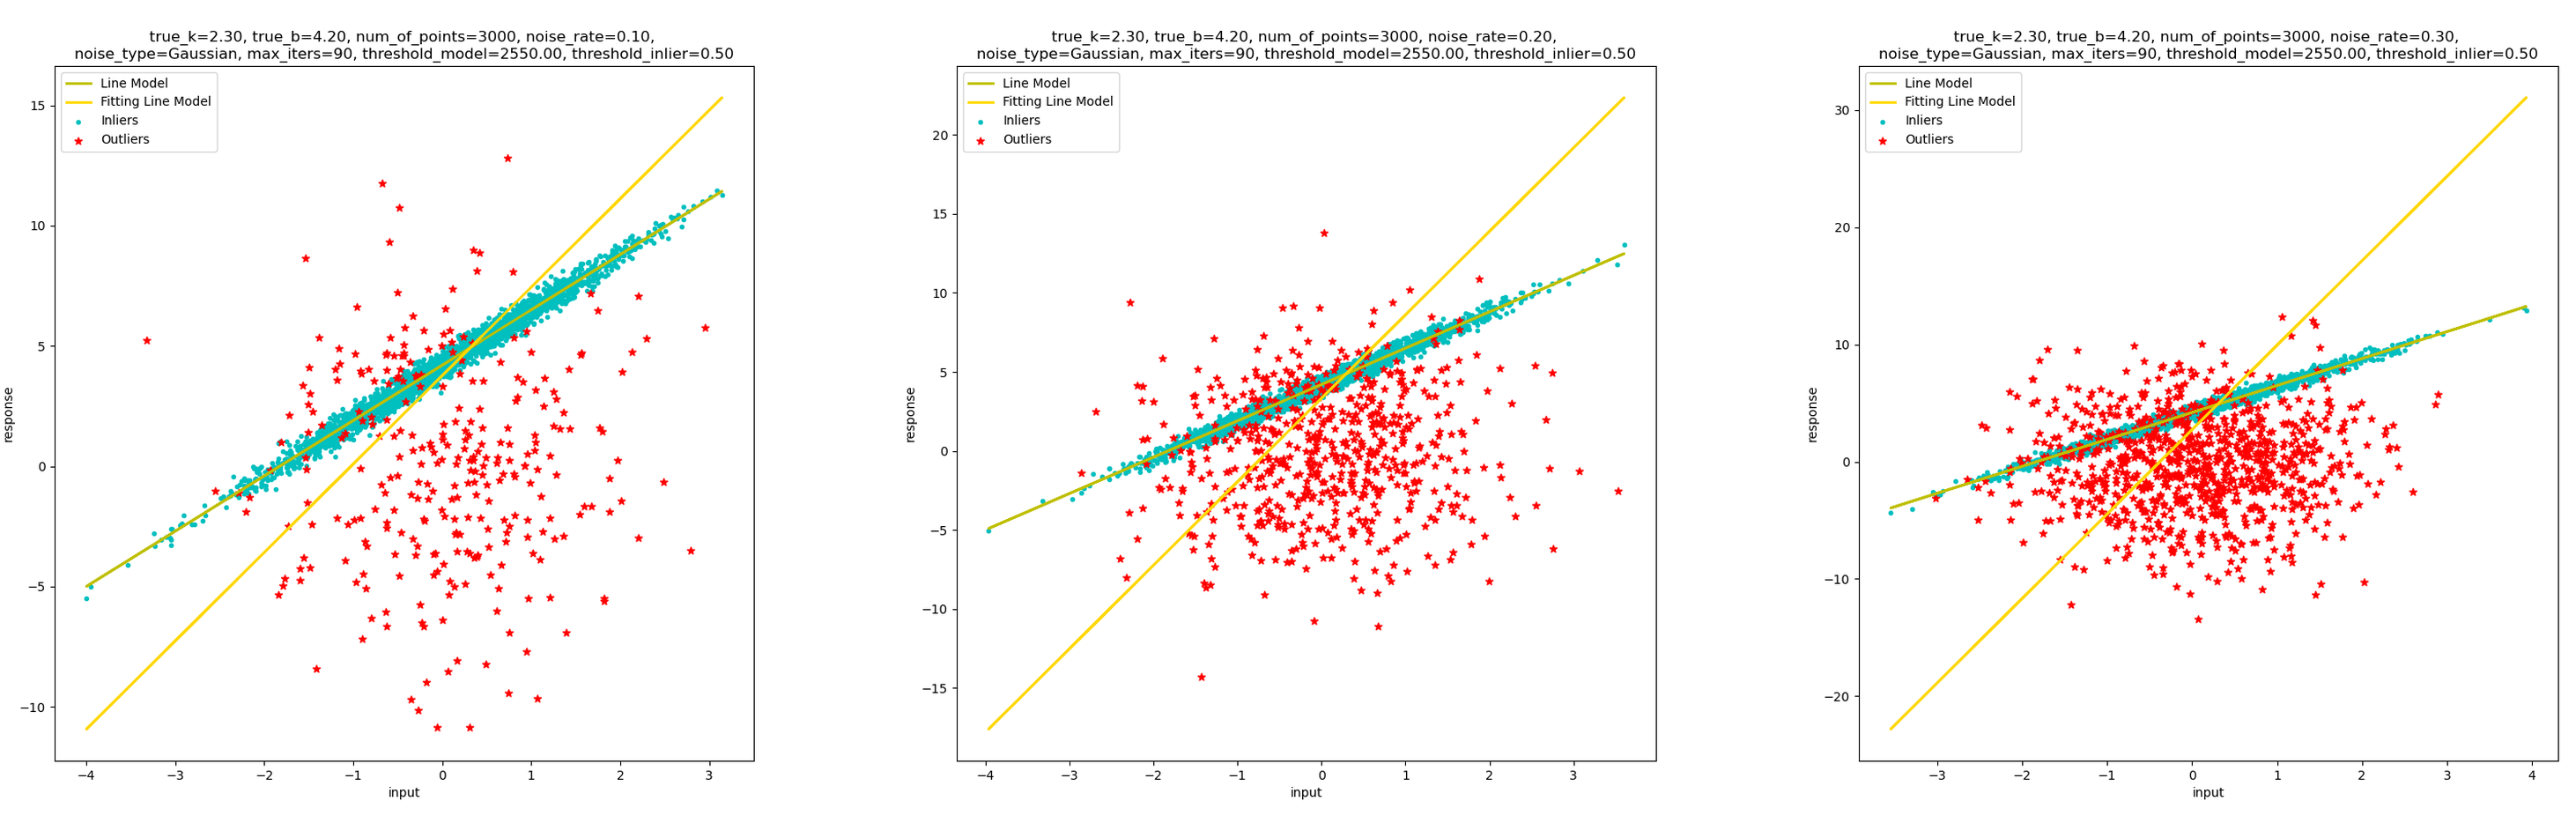
\includegraphics[scale=0.1]{./image/test_noise_rate_Gaussian.png}
  \caption{RANSAC Test different Gaussian noise rate} \label{fig:eg}
\end{figure}

从左到右分别是在均匀噪音率0.1,0.2,0.3的数据集上拟合的效果图
\begin{figure}[H]
  \centering
  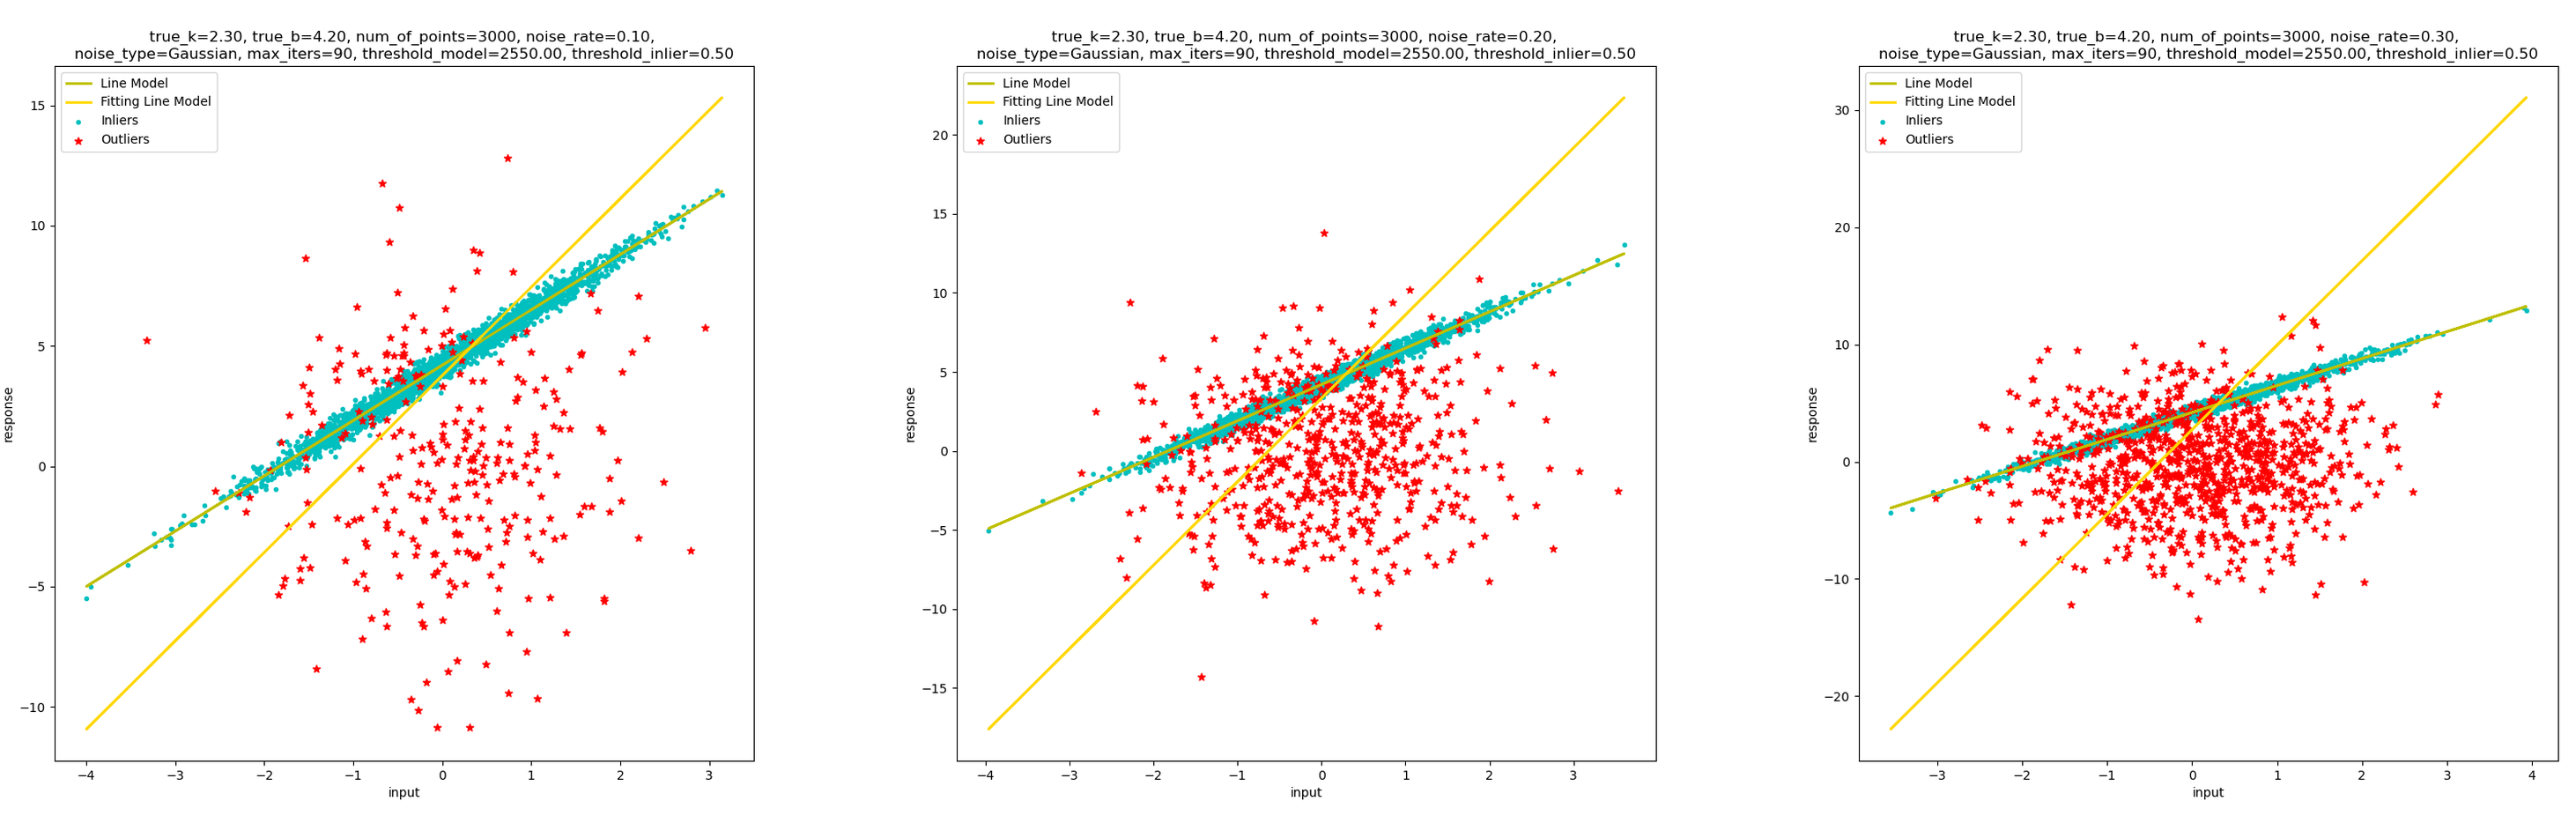
\includegraphics[scale=0.1]{./image/test_noise_rate_Gaussian.png}
  \caption{RANSAC Test different Uniform noise rate} \label{fig:eg}
\end{figure}
\begin{table}[h]
  \centering
  \captionnamefont{\wuhao\bf\heiti}
  \captiontitlefont{\wuhao\bf\heiti}
  \caption{测试结果总览} \label{tab:eg1}
  \liuhao
  \begin{tabular}{cccccc}
  \toprule
  {编号} & {噪音比例} & {噪音类型} & {内点率} & {均方距离} & {时间/s} \\
  \midrule 
  1 & 0.1 & Gaussian & 0.865 & 0.456 & 1.31 \\
  2 & 0.2 & Gaussian & 0.695 & 0.695 & 0.66 \\
  3 & 0.3 & Gaussian & 0.593 & 0.789 & 0.70\\
  4 & 0.1 & Uniform  & 0.917 & 0.376 & 0.70\\
  5 & 0.2 & Uniform  & 0.756 & 0.582 & 0.95\\
  6 & 0.3 & Uniform  & 0.670 & 0.713 & 0.66\\
  \bottomrule
  \end{tabular}
\end{table}
我们可以发现,无论是高斯噪音还是均匀噪音,随着噪音率的增大,RANSAC的拟合误差也在增大,这也表明RANSAC在面对程度较高的噪音条件下,会出现较大拟合误差;与此同时我们发现RANSAC对均匀噪声的抗噪能力较强,在同等噪声比例下,能显示较高的准确率

\paragraph{不同内点阈值拟合效果比较}

从左到右是在带有高斯噪音数据集上分别以0.1,0.2,0.3为内点阈值拟合的效果图
\begin{figure}[H]
  \centering
  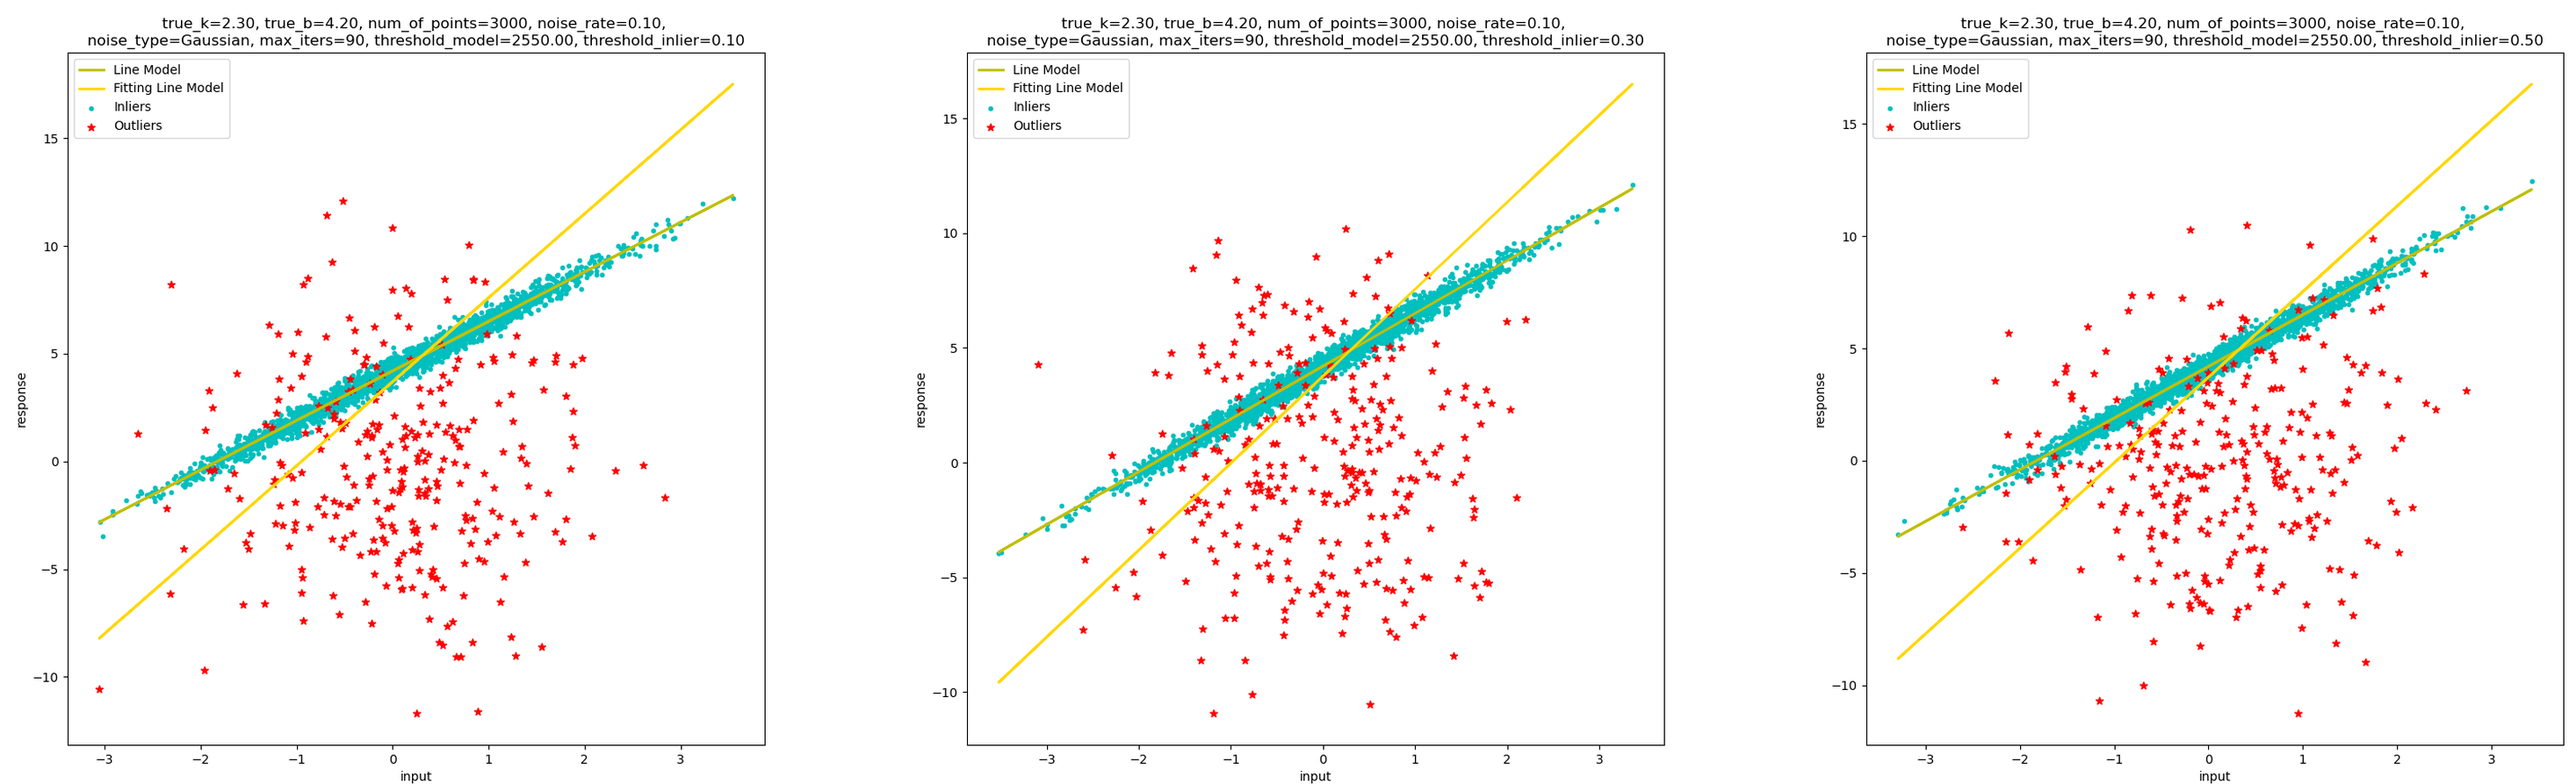
\includegraphics[scale=0.1]{./image/test_threshold_Gaussian.png}
  \caption{RANSAC Test different threshold with Gaussian noise} \label{fig:eg}
\end{figure}
从左到右是在带有平滑噪音数据集上分别以0.1,0.2,0.3为内点阈值拟合的效果图
\begin{figure}[H]
  \centering
  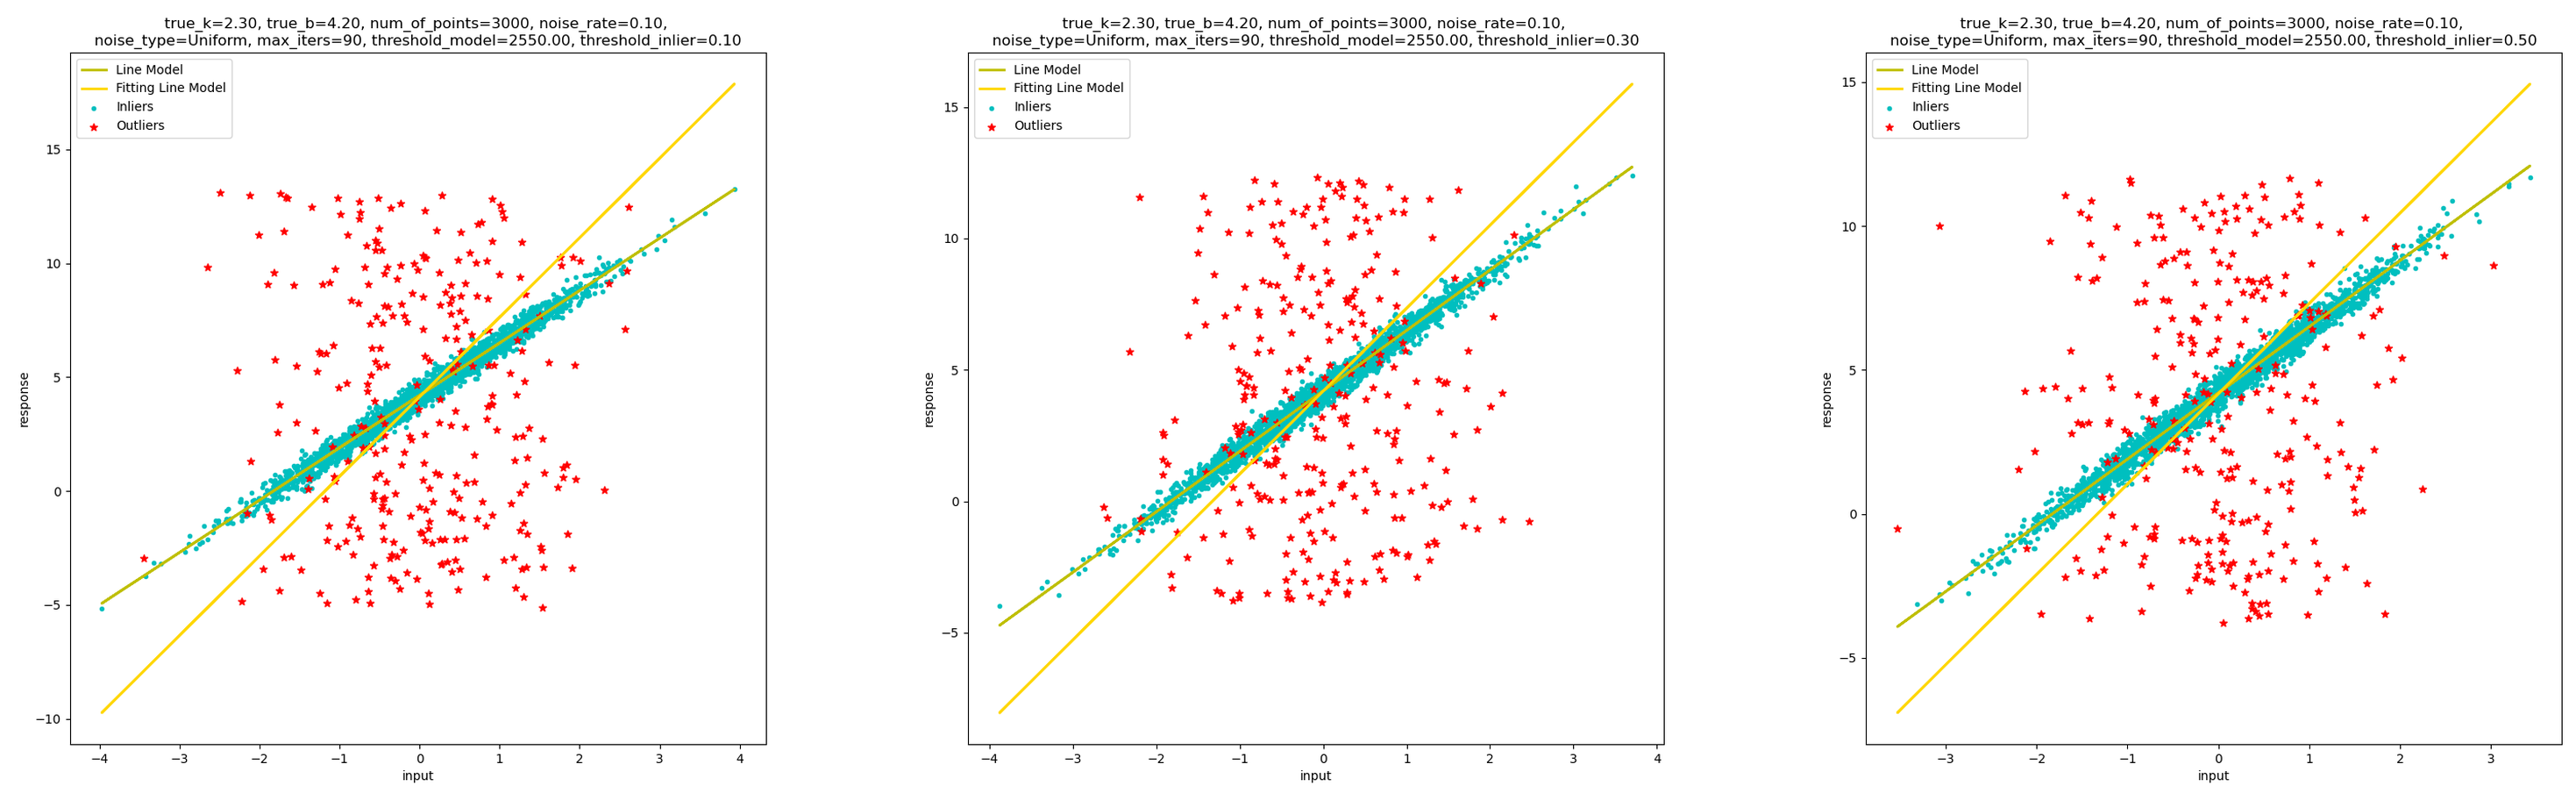
\includegraphics[scale=0.1]{./image/test_threshold_Uniform.png}
  \caption{RANSAC Test different threshold with Uniform noise} \label{fig:eg}
\end{figure}

\begin{table}[h]
  \centering
  \captionnamefont{\wuhao\bf\heiti}
  \captiontitlefont{\wuhao\bf\heiti}
  \caption{测试结果总览} \label{tab:eg1}
  \liuhao
  \begin{tabular}{cccccc}
  \toprule
  {编号} & {噪音类型} & {内点阈值} & {内点率} & {均方距离} & {时间/s} \\
  \midrule 
  1 & Gaussian & 0.1 & 0.495 & 0.474 & 0.62 \\
  2 & Gaussian & 0.3 & 0.766 & 0.443 & 0.62 \\
  3 & Gaussian & 0.5 & 0.866 & 0.446 & 0.68\\
  4 & Uniform  & 0.1 & 0.585 & 0.428 & 0.70\\
  5 & Uniform  & 0.3 & 0.880 & 0.336 & 0.63\\
  6 & Uniform  & 0.5 & 0.920 & 0.327 & 0.65\\
  \bottomrule
  \end{tabular}
\end{table}
我们可以发现,无论是均匀噪声还是高斯噪声,提高内点阈值,都可以大幅度提高准确率;但相比于高斯噪声,在均匀噪声的条件下,效果更好
\paragraph{不同模型阈值拟合效果比较}

从左到右是在带有高斯噪音数据集上分别以0.75,0.85,0.95为模型阈值拟合的效果图
\begin{figure}[H]
  \centering
  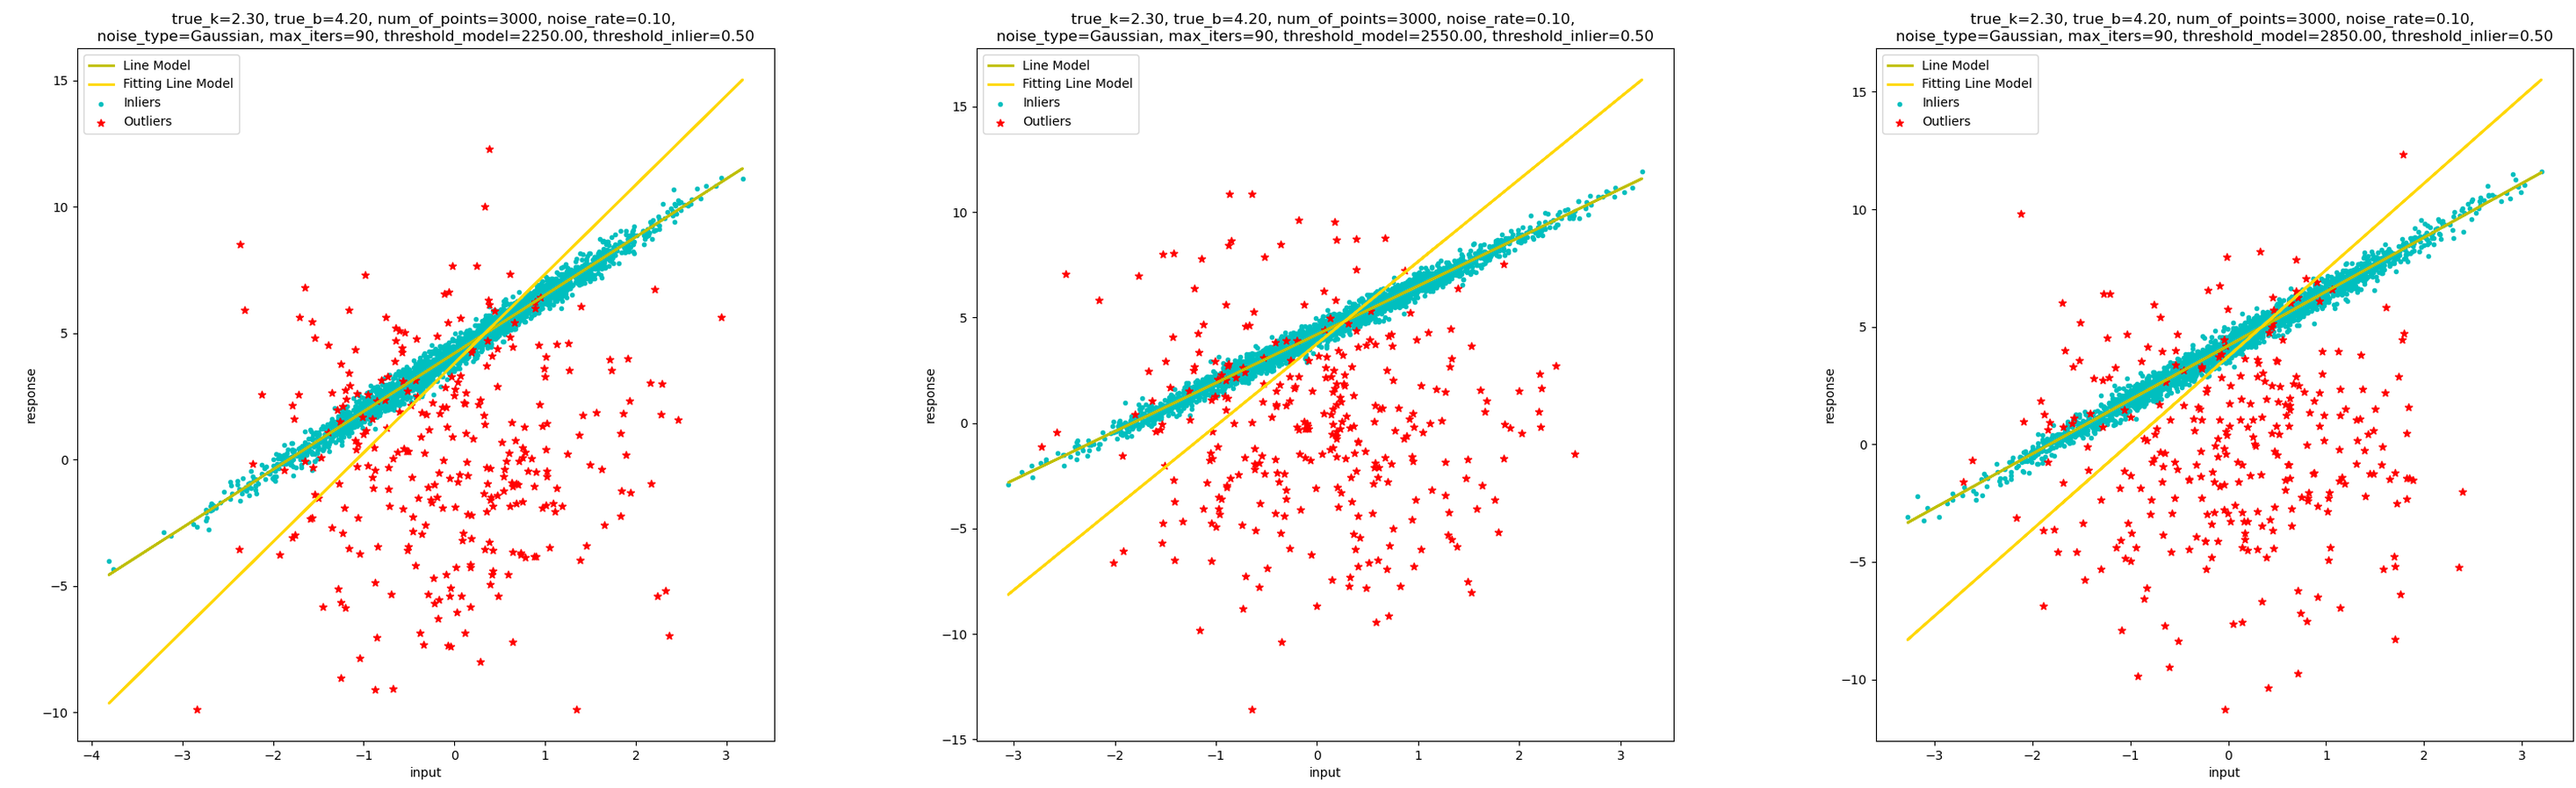
\includegraphics[scale=0.1]{./image/test_threshold_model_Gaussian.png}
  \caption{RANSAC Test different threshold with Gaussian noise} \label{fig:eg}
\end{figure}
从左到右是在带有平滑噪音数据集上分别以0.75,0.85,0.95为模型阈值拟合的效果图
\begin{figure}[H]
  \centering
  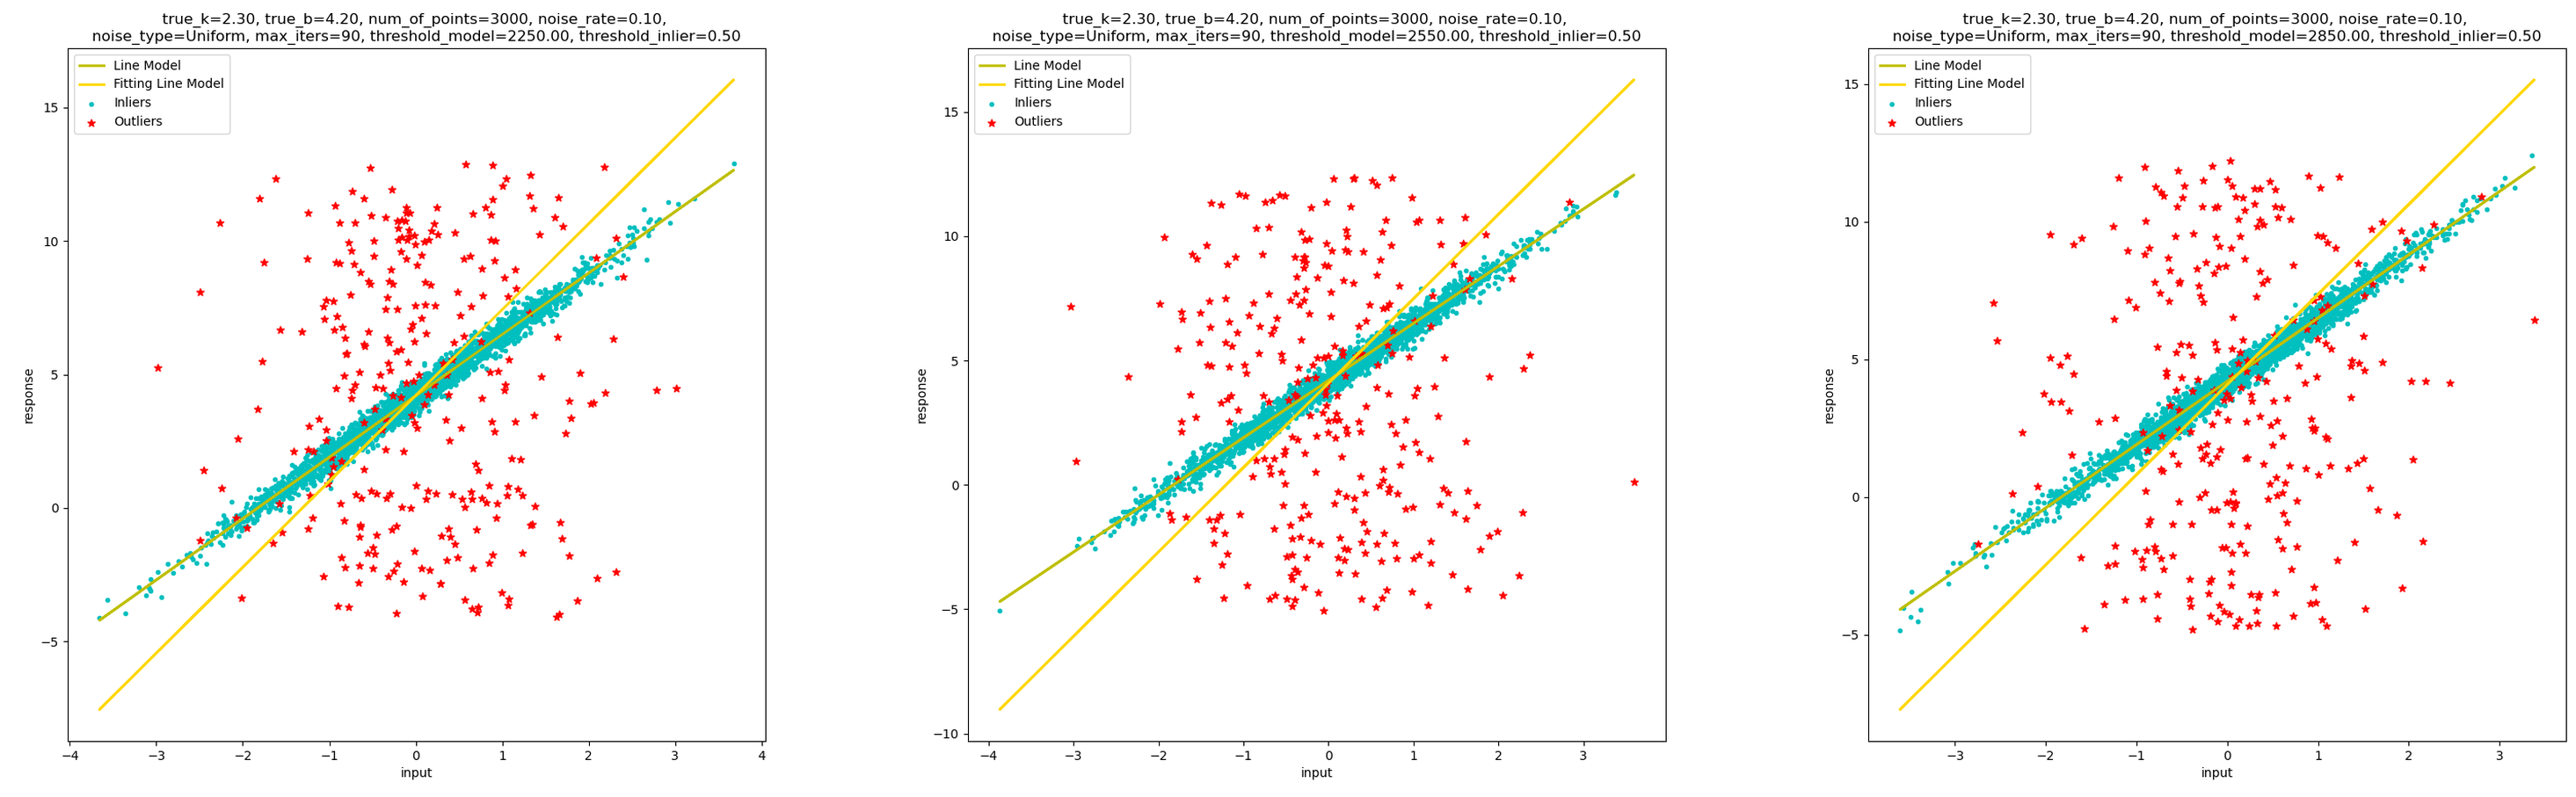
\includegraphics[scale=0.1]{./image/test_threshold_model_Uniform.png}
  \caption{RANSAC Test different threshold with Uniform noise} \label{fig:eg}
\end{figure}
\newpage
\begin{table}[h]
  \centering
  \captionnamefont{\wuhao\bf\heiti}
  \captiontitlefont{\wuhao\bf\heiti}
  \caption{测试结果总览} \label{tab:eg1}
  \liuhao
  \begin{tabular}{cccccc}
  \toprule
  {编号} & {噪音类型} & {模型阈值} & {内点率} & {均方距离} & {时间/s} \\
  \midrule 
  1 & Gaussian & 0.75 & 0.888 & 0.423 & 0.63 \\
  2 & Gaussian & 0.85 & 0.848 & 0.461 & 0.64 \\
  3 & Gaussian & 0.95 & 0.865 & 0.445 & 0.65\\
  4 & Uniform  & 0.75 & 0.913 & 0.369 & 0.63\\
  5 & Uniform  & 0.85 & 0.901 & 0.399 & 0.60\\
  6 & Uniform  & 0.95 & 0.904 & 0.362 & 0.65\\
  \bottomrule
  \end{tabular}
\end{table}
我们可以发现,对于模型阈值的调节不会特别影响准确率,但随着模型阈值的升高,模型的准确率也在提高
% \begin{figure}
%   \begin{minipage}[t]{0.33\linewidth}
%   \centering
%   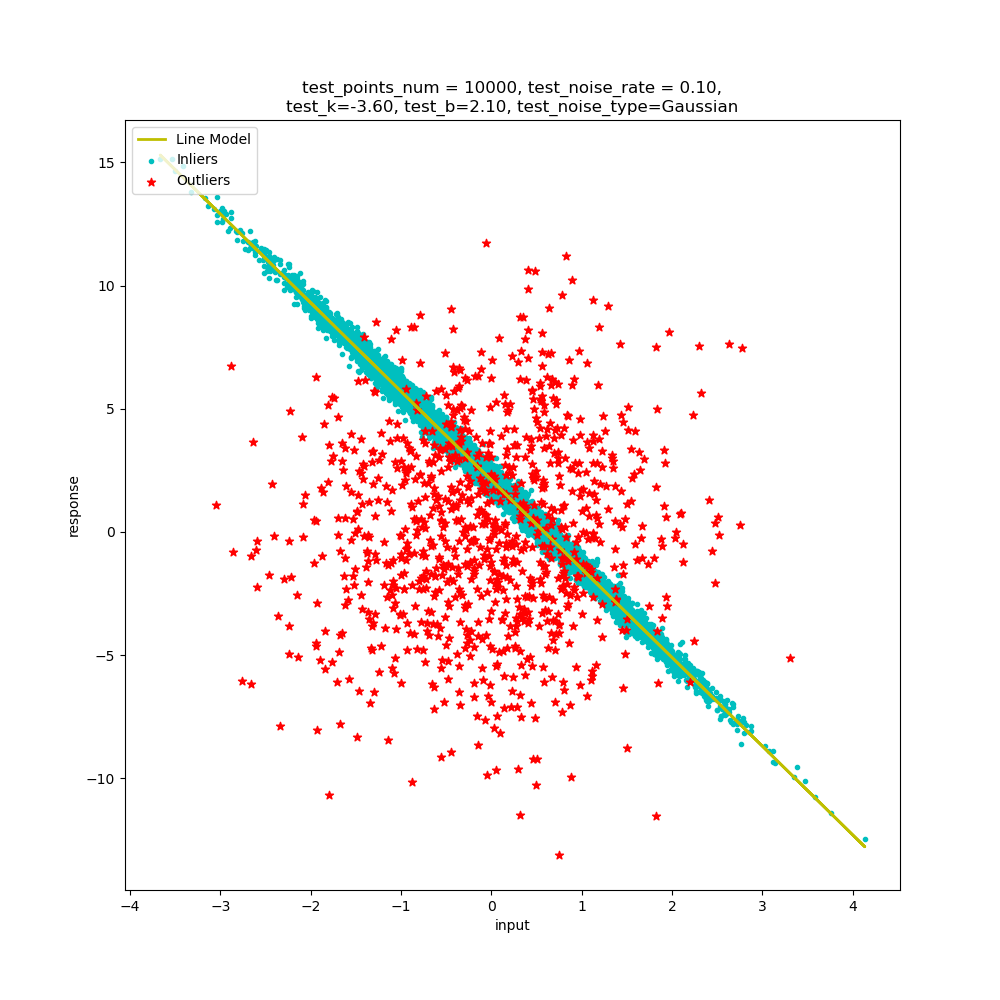
\includegraphics[width=0.85\linewidth]{./image/test_gen_data_(0.10, Gaussian).png}
%   \caption{300 Gaussian Noise}
%   \label{fig:side:a}
%   \end{minipage}%
%   \begin{minipage}[t]{0.33\linewidth}
%   \centering
%   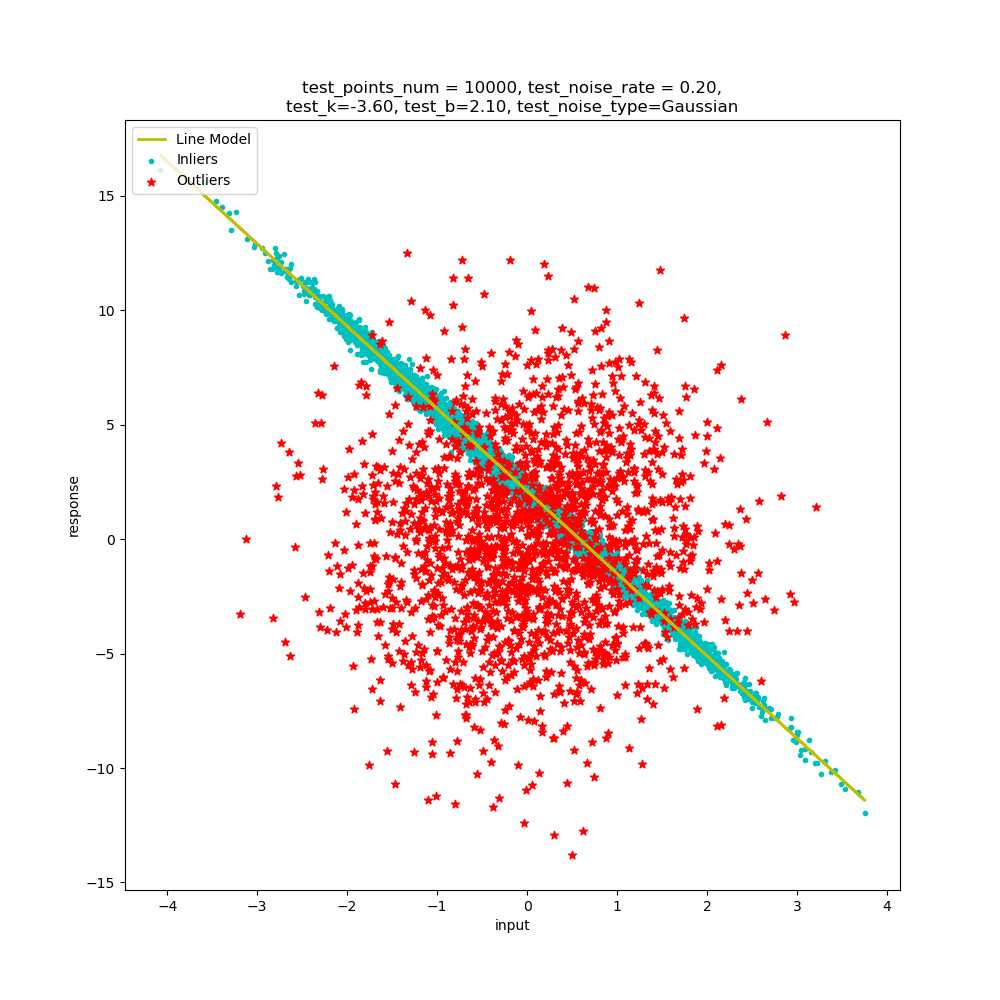
\includegraphics[width=0.85\linewidth]{./image/test_gen_data_(0.20, Gaussian).png}
%   \caption{600 Gaussian Noise}
%   \label{fig:side:b}
%   \end{minipage}
%   \begin{minipage}[t]{0.33\linewidth}
%     \centering
%     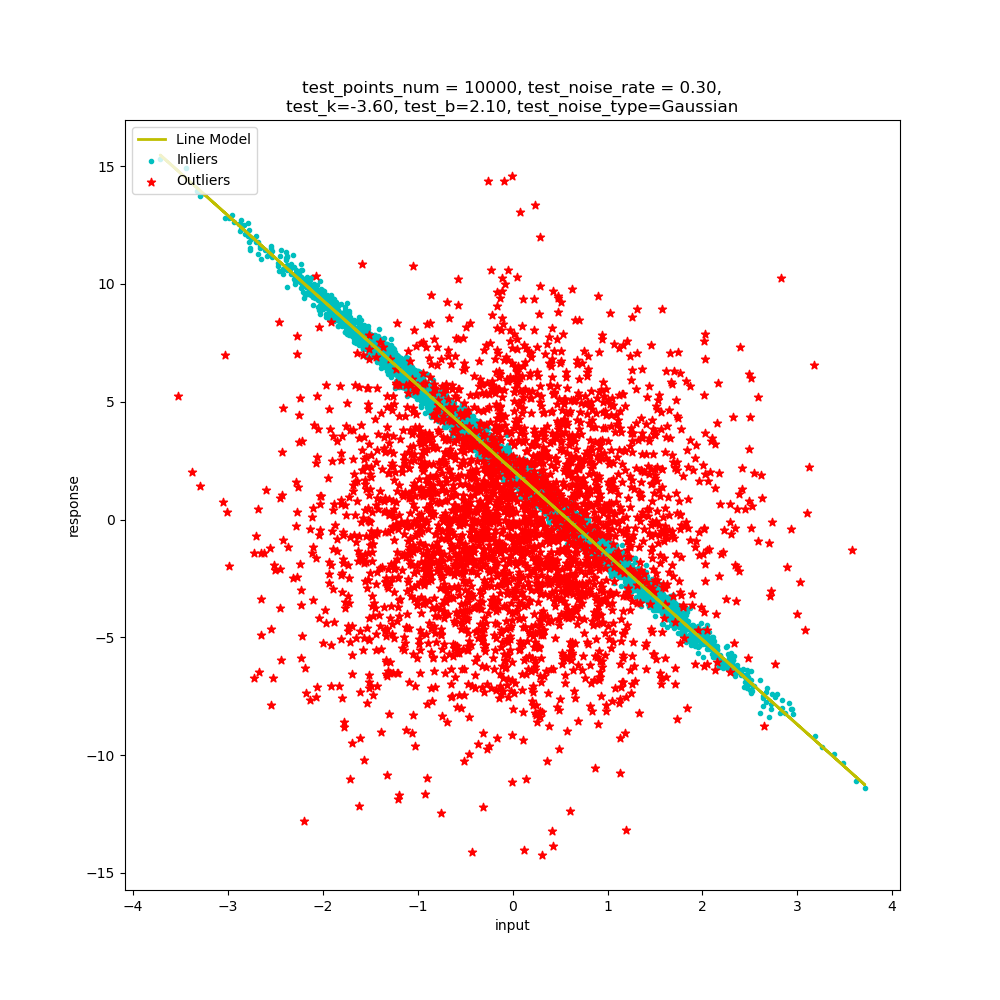
\includegraphics[width=0.85\linewidth]{./image/test_gen_data_(0.30, Gaussian).png}
%     \caption{900 Gaussian Noise}
%     \label{fig:side:c}
%     \end{minipage}
%   % \caption{3000 points with Gaussian Noise}
%   % \label{fig:eg} %% label for entire figure
% \end{figure}

\subsubsection{自适应调节最大迭代数测试}
\begin{table}[h]
  \centering
  \captionnamefont{\wuhao\bf\heiti}
  \captiontitlefont{\wuhao\bf\heiti}
  \caption{测试结果总览} \label{tab:eg1}
  \liuhao
  \begin{tabular}{cccc}
  \toprule
  {编号} & {抽样样本数} & {最大迭代数} & {时间/s} \\
  \midrule 
  1 & 10 & 7 & 0.04\\
  2 & 20 & 19 & 0.08\\
  3 & 30 & 46 & 0.20\\
  4 & 40 & 106 & 0.45\\
  5 & 50 & 233 & 0.99\\
  \bottomrule
  \end{tabular}
\end{table}

\section{总结展望}
在本次实验中,我通过手动实现了RANSAC模型,从而对RANSAC相关算法都有了更深的理解,这将为后续实现更复杂的拟合算法打下坚实的基础。同时,我也从中发现了RANSAC的许多不足,例如参数较多、计算量大、收敛困难。但总体而言最终的结果还是令人欣慰的。

而由于时间原因,本次实验并未实现平面拟合。在后续学习生涯中,若有机会,将会尝试实现平面拟合的相关算法。


% \subsection{往届学生报告中常见问题与不足}
% 正文内容正文文字五号宋体正文内容正文文字五号宋体正文内容正文文字五号宋体正文内容正文文字五号宋体正文内容正文文字五号宋体正文内容正文文字五号宋体正文内容。
% \subsubsection{三级标题}
% \subsubsection{只给数据和结果,没有对结果所反映的物理规律做理论分析及数据误差分析;}
% \subsubsection{数据及结果直接给出,没有必要的实验条件说明和所用物理计算公式;}
% \subsubsection{结果以图、表给出时,图、表不规范(缺少坐标分度、物理量及其单位等);}
% 正文内容正文文字五号宋体正文内容正文文字五号宋体正文内容正文文字五号宋体正文内容正文文字五号宋体正文内容正文文字五号宋体正文内容正文文字五号宋体正文内容。
% \subsection{报告中公式、字母的规范写法}
% 公式全文统一编号,如公式为
% \begin{equation}\label{EQ1}
% \frac{\partial u}{\partial x}+\frac{\partial v}{\partial y}+\frac{\partial w}{\partial z}=0
% \end{equation}
% 式中,u×××(单位);v××(单位);w是××(单位)。

% 对于公式,应全文统一连续编号,如式\eqref{EQ1}……一般情况下,需要引用的或重要的公式才编号。在文中引用时,用“式(编号)”表示。
% 后文不再提及的,可以不编号。如
% \begin{equation*}
% 1 + 1 + 3 = 5
% \end{equation*}

% 对于公式中首次出现的量的符号,按照其在式中出现的顺序,用准确、简洁的语句对其进行逐一解释。公式中变量应尽量避免复合上下角标的使用;尽量少用3层关系的上下标,同时应尽量减少不必要的公式推导。

% \subsection{报告中图的规范要求}
% 插图全文顺序编号。插图内容应与正文内容密切结合,每幅图前都应有相应的引出或介绍文字。图形应保证线条清晰,图形大小应适应版面要求,合理布局,图内如有标注或说明性文字时应清晰可辨。图中除了物理量符号及单位外一律用中文,同一图中的不同曲线应用不同线型表示。插图分辨率要大于600PPI。

% 正文文字中先见文,后见图,图号全文统一按顺序编号,如图\ref{fig:eg}所示。图中文字为6号,图线必须清晰可辨坐标轴的物理量和单位不可缺。


% \begin{figure}[H]
% \centering
% 
\includegraphics[width=0.8\linewidth]{./image/5000choyen.png}
% \caption{图片示例} \label{fig:eg}
% \end{figure}


% \subsection{报告中表的规范}
% 推荐使用标准“三线表”(如表\ref{tab:eg1}所示。),内容易混淆时可加辅助线进行辅助说明。按表格在文中出现的顺序,用阿拉伯数字对其进行编号,全文顺序编号。应有相应的表题且每个表格前都应有相应的引出或介绍文字。

% 图、表应在文中有相应表述,即图、表的号应在文中引出,以先见文后见图、表为原则。每个图、表都必须有图名、表名,并且有编号。图号、表号应全文统一连续排列,即,应按照图1、图2……排列不应按小结编号。图片中的文字、线条应当清晰可辨,图片像素(DPI)在300以上。
% 表格推荐采用全线表,表头中使用量符号/量单位形式。如表\ref{tab:eg2}所示。

% \begin{table}[h]
% \centering
% \captionnamefont{\wuhao\bf\heiti}
% \captiontitlefont{\wuhao\bf\heiti}
% \caption{三线表示例} \label{tab:eg1}
% \liuhao
% \begin{tabular}{cccc}
% \toprule
% {编号} &  {直径}/\si{\metre} & {静温}/\si{\kelvin} & {时间}/min\\
% \midrule 
% 4 & 0.0349 & 268.15 & 30\\
% 5 & 0.01905 & 268.15 & 30\\
% \bottomrule
% \end{tabular}
% \end{table}

% \begin{table}[h]
% \centering
% \captionnamefont{\wuhao\bf\heiti}
% \captiontitlefont{\wuhao\bf\heiti}
% \caption{全线表示例} \label{tab:eg2}
% \liuhao
% \begin{tabular}{|c|c|c|c|c|}
% \hline
% U/V & I/mA & v/km·h$^{-1}$ & x/mm & p/MPa \\ \hline
% \textit{12} & \textit{30} & \textit{80} & \textit{55} & \textit{110} \\ \hline
% \textit{24} & \textit{34} & \textit{90} & \textit{60} & \textit{111} \\ \hline
% \end{tabular}
% \end{table}

% \subsection{报告中英文缩略语的规范}
% 文中的英文缩略语应在首次出现时给出中文含义以及英文全称后再使用。例如,全球定位系统(Global Positioning System,GPS)。


% \subsection{外文字母}
% \subsubsection{斜体外文字母用于表示量的符号,主要用于下列场合}

% \begin{enumerate}
% \renewcommand{\labelenumi}{(\theenumi)}
% \item 变量符号、变动附标及函数。
% \item 用字母表示的数及代表点、线、面、体和图形的字母。
% \item 特征数符号,如Re (雷诺数)、Fo (傅里叶数)、Al (阿尔芬数)等。
% \item 在特定场合中视为常数的参数。
% \end{enumerate} 

% \subsubsection{正体外文字母用于表示名称及与其有关的代号,主要用于下列场合}
% \begin{enumerate}
% \renewcommand{\labelenumi}{(\theenumi)}
% \item 有定义的已知函数(例如$\sin$, $\exp$, $\ln$等)。
% \item 其值不变的数学常数(例如$\mathrm{e} = 2.718 281 8\cdots)$及已定义的算子。
% \item 法定计量单位、词头和量纲符号。
% \item 数学符号。
% \item 化学元素符号。
% \item 机具、仪器、设备和产品等的型号、代号及材料牌号。
% \item 硬度符号。
% \item 不表示量的外文缩写字。
% \item 表示序号的拉丁字母。
% \item 量符号中为区别其他量而加的具有特定含义的非量符号下角标。
% \end{enumerate} 

% \section{结~~论}
% 用准确、精炼的语言归纳总结使用的方法以及研究结果。

% 说明研究的创新价值和应用价值,包括对科技工作者的研究的价值和对产业发展的价值。

% 可说明自己做本实验的总结、收获和体会,对实验中发现的问题提出自己的建议。


% %%%%%%%%%%%%%%%%%%%%%%%%%%%%%%%%%%%%%%%%%%%%%%%%%%%%%%%%%%%%%%%%
% %  参考文献
% %%%%%%%%%%%%%%%%%%%%%%%%%%%%%%%%%%%%%%%%%%%%%%%%%%%%%%%%%%%%%%%%
% %  参考文献按GB/T 7714-2015《文后参考文献著录规则》的要求著录. 
% %  参考文献在正文中的引用方法:\cite{bib文件条目的第一行}

% \renewcommand\refname{\heiti\wuhao\centerline{参考文献}\global\def\refname{参考文献}}
% \vskip 12pt

% \let\OLDthebibliography\thebibliography
% \renewcommand\thebibliography[1]{
%   \OLDthebibliography{#1}
%   \setlength{\parskip}{0pt}
%   \setlength{\itemsep}{0pt plus 0.3ex}
% }

% {
% \renewcommand{\baselinestretch}{0.9}
% \liuhao
% \bibliographystyle{gbt7714-numerical}
% \bibliography{./example}
% }


\end{document}
